\begin{table}[H]
    {\renewcommand{\arraystretch}{1.2}%
    \setlength{\tabcolsep}{0.3em}%
\begin{tabular}{bababab}
\toprule

\rowcolor{white} \null &
\textbf{Synthetic$_{\mathbf{\mathcal{F}}}$} & \textbf{Synthetic$_{\mathbf{\mathcal{\beta}}}$} &
\textbf{Lehrpfad$_{\mathbf{\mathcal{F}}}$} & \textbf{Lehrpfad$_{\mathbf{\mathcal{\beta}}}$} &
\textbf{Office$_{\mathbf{\mathcal{F}}}$} & \textbf{Office$_{\mathbf{\mathcal{\beta}}}$} \\
\midrule

\rowcolor{lightgray}
\textbf{Keypoint Count} &
    \num{217505} & \num{44221} &
    \num{2168190} & \num{2198592} &
    \num{171000} & \num{171000} \\
\textbf{Correspondences} &
    \num{96371} & \num{26455} &
    \num{297949} & \num{222495} &
    \num{43037} & \num{36309} \\
\rowcolor{lightgray}
\textbf{True Positives} &
    \num{76603} & \num{22179} &
    \num{110339} & \num{35387} &
    \num{24025} & \num{15455} \\
\textbf{False Positives} &
    \num{59032} & \num{8865} &
    \num{648603} & \num{651091} &
    \num{48868} & \num{48697} \\
\rowcolor{lightgray}
\textbf{False Negatives} &
    \num{19768} & \num{4276} &
    \num{187610} & \num{187108} &
    \num{19012} & \num{20854} \\

\bottomrule
\end{tabular}

    }
    \caption{Performance indicators for the default configuration of the SIFT algorithm on the different datasets.}
\end{table}
The final feature detection algorithm evaluate is \acrshort{akaze}, that is again closer to \acrshort{sift} for the keypoint detector design compared to \acrshort{orb}.
\acrshort{akaze} results approximatly one order of magnitude more detected keypoints and correspondences compared to \acrshort{sift}.
Its keypoints characteristics show expected results (Appendix~\ref{sec:akaze_stats}).
Compared to \acrshort{sift} the detection does not result in as similar diverse keypoint sizes and the response is narrower with a stronger skew towards small responses.

The \acrshort{mldb} descriptor shows separation between true positive and false positives across the datasets and feature images.
This indicates good performance of the binary descriptor.
Additionally it reaffirms the finding of \acrshort{orb}'s \acrshort{brief} descriptor showing separation potential.
The enhancement in \acrshort{mldb} solidifies the tendency though.
\begin{figure}[htp]
\begin{subfigure}[t]{0.45\linewidth}
    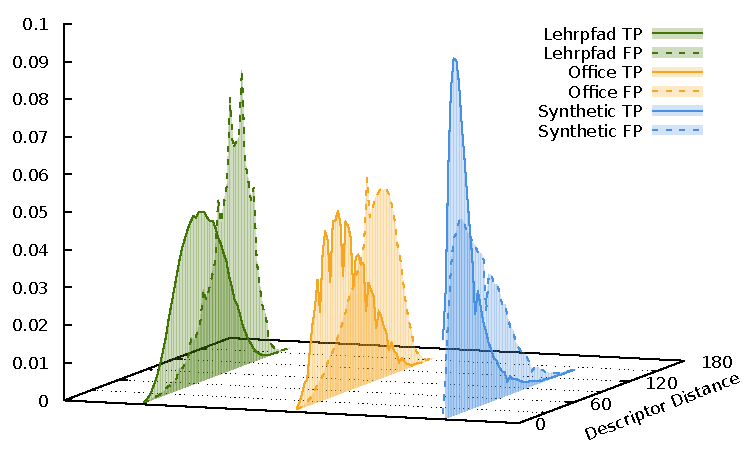
\includegraphics[width=\linewidth]{chapter06/results/AKAZE/flexion/descriptor_distances.pdf}%
    \caption{\gls{flexion-image} Descriptor Distances}
\end{subfigure}\quad
\begin{subfigure}[t]{0.45\linewidth}
    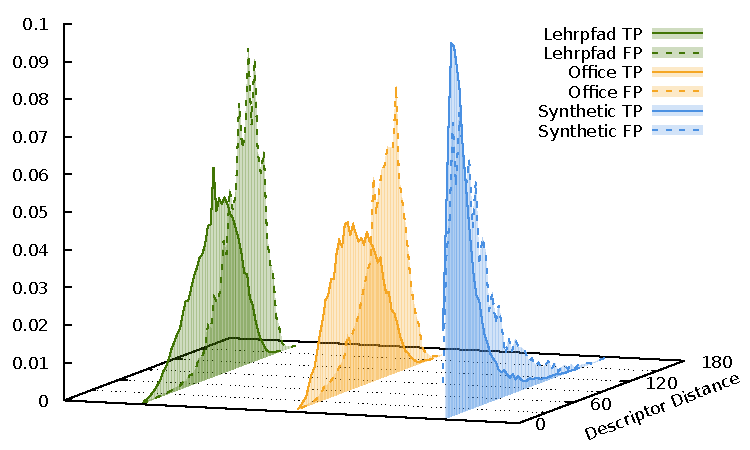
\includegraphics[width=\linewidth]{chapter06/results/AKAZE/bearing/descriptor_distances.pdf}%
    \caption{\gls{bearing-angle-image} Descriptors Distances}
\end{subfigure}
\end{figure}
The ROC graph in Figure~\ref{fig:roc_akaze} shows, that \acrshort{akaze} can perform quiet reasonable across all datasets.
For the \glspl{flexion-image} there exists a configuration for each dataset with significantly higher true positive rate than false positive rate.
The top performers for each dataset are the configurations using only the best 400 keypoints for matching, regardless of filtering.
Applying additional heuristics in matching, like a maximum matching distance, will certainly improve the ratio of true positives to false positives further.
The backprojections in Appendix~\ref{sec:backprojections_akaze} show the higher amount of keypoints compared to \acrshort{sift}.
But bad scale coverage leads to unsatisfying keypoint for the \emph{Laserscan} dataset.
There, \acrshort{sift} has clear qualitative advantages over \acrshort{akaze}, because its keypoints cover the whole scan.
\begin{figure}[htp]
\begin{subfigure}[t]{0.45\linewidth}
    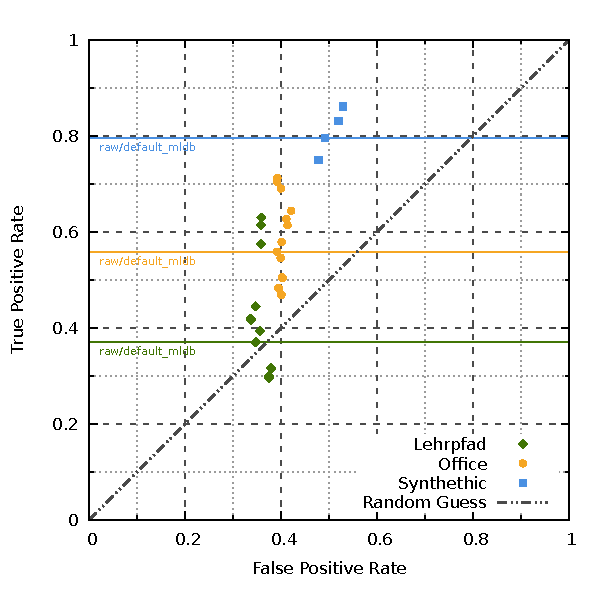
\includegraphics[width=\linewidth]{chapter06/results/AKAZE/flexion/roc.pdf}%
    \caption{Flexion Image ROC}
\end{subfigure}\quad
\begin{subfigure}[t]{0.45\linewidth}
    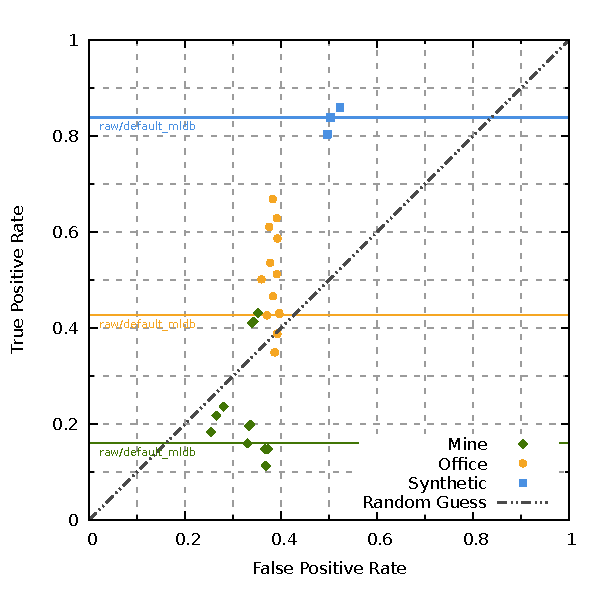
\includegraphics[width=\linewidth]{chapter06/results/AKAZE/bearing/roc.pdf}
    \caption{Bearing-Angle Image ROC}
\end{subfigure}
    \caption{ROC graph for \acrshort{akaze}.}\label{fig:roc_akaze}
\end{figure}
